%Template generated by Ben Manning
%Purdue University
%btmannin@purdue.edu
%Last modified: 7/7/2021


\documentclass[notitlepage, 12pt]{report}  %The document class will setup a lot of basic formatting.  Report class will start with justifying paragraphs setup your different types of sections.

%Different packages allow you to add more functions that will make your time in LaTeX easier.
\usepackage{amsmath}
\usepackage{graphicx} % pictures
\usepackage{caption}
\usepackage{url}
\usepackage{circuitikz} % circuit drawer

%\usepackage{biblatex} %Imports biblatex package
\usepackage[style=numeric]{biblatex}
\addbibresource{bib.bib}

\usepackage[top=2cm, bottom=2cm, left=2cm, right=2cm]{geometry}

\graphicspath{ {./images/} }

\title{Experiment 1 Report}

\begin{document}
%Everything needs to begin and end.  


\begin{center}
\large \textbf{Experiment 1 Report} \\ %\large and \small can help make text sizes vary throughout your document.
%\textbf will bold the text that is in the curly brackets
\small 
Andrew Lykken\\
Anna Kishnani\\
19 January 2023\\
Section 004 (Abraham Yakisan)\\
%\rule{500pt}{.1pt} 

\end{center}

% space between title and abstract
\vspace{4in}


\begin{abstract}
abstract here 
\end{abstract}

\newpage

% ----------------BEGIN TASKS--------------------- %

% ----- TASK 1 ----- %

\section*{Task 1} %Each task has a section including (but not limited to) Objective, 
% Procedure, Results / Calculations, Conclusions


\subsection*{Objective}
\indent\indent This section will demonstrate basic measurement techniques and functions learned in ECE 20007, using 
the lab instruments provided, including an oscilloscope, waveform generator, digital multimeter (DMM), 
and variable DC power supply. 

\subsection*{Procedure}
\indent\indent For testing purposes, the function:
\begin{equation}
    2 \sin(2\pi 750t)
\end{equation}

was generated with the waveform generator.\\

The waveform generator was connected to one channel of an oscilloscope, and adjusted so that the signal 
was stable and reasonably sized within the window.\\


\noindent On the oscilloscope, 

\begin{itemize} % bullet points

    \item{The window was resized horizontally such that more periods of the wave were visible.}

    \item{The trigger level was modified between -4V and 4V.}

    \item{The horizontal and vertical offsets of the signal were modified.}
    
\end{itemize}

After recording findings, the DC power supply was set to 3.3V. The AC and DC RMS values were measured through 
the DMM.\\


\subsection*{Results / Calculations}

\indent\indent Each control serves a different function for manipulating the signal viewed on the oscilloscope. \\

The horizontal scale adjustment knob determines the scale of time on the oscilloscope's horizontal axis. 
This can vary widely, depending on what signal is being passed to the oscilloscope's input channel. 
An analogy for what this control does is that it ``squishes'' or ``stretches'' the view of the signal being measured. \\

The trigger level is a set voltage that the oscilloscope looks for when measuring signals to create stability in the
image shown. The level of the trigger determines at what voltage and time the signal lines up with.\\

Below is a screenshot containing the signal displayed in normal mode.

\begin{center}
    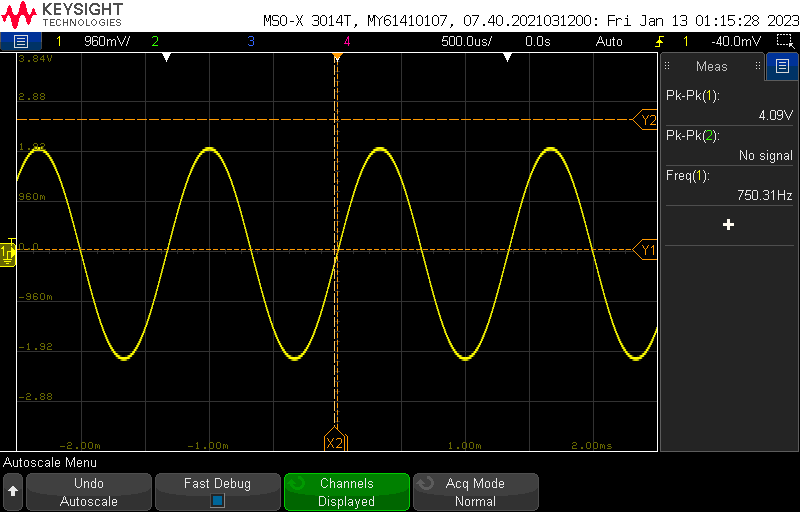
\includegraphics[scale=0.5]{scope1.png}
\end{center}


The offsets control the position of the signal in the viewing window. The vertical offset can move the signal up 
or down on the graph, where ground is shown with a marker on the vertical axis to the left of the signal. The
horizontal offset moves the signal in time as shown. The signal appears to move left or right, indicating a 
change in time measurements, being slightly ahead or behind where the original location was. \\

For using the DMM and DC power supply, the DC RMS and AC RMS values were measured to be:

\begin{equation}
    DC_{RMS} = 3.3005V
\end{equation}

\begin{equation}
    AC_{RMS} = 0.003V
\end{equation}

Knowing the nominal value for the $DC_{RMS}$ being 3.3V, the following error calculation can be achieved:

\begin{equation}
    \%_{err} = \frac{|V_{meas} - V_{ideal}|}{V_{ideal}} = \frac{|DC_{RMS,meas} - DC_{RMS,nominal}|}{DC_{RMS,nominal}} = 
    \frac{|3.305V - 3.3V|}{3.3V} = 0.15\%
\end{equation}


\subsection*{Conclusions}

\indent\indent This task explored the techniques and adjustments that can be made when measuring a circuit or signal,
and how such measurements can impact the readability and usefulness of the tools used. On the oscilloscope, 
signals can be manipulated in many ways to make them more readable and measurable to a user. The DMM has
multiple modes that can be used to measure different types of signals, differentiated by being AC or DC 
values.\\


% ----- TASK 2 ----- %

\section*{Task 2}

\subsection*{Objective}
\indent\indent This section will explore a CMOS inverter and its voltage transfer characteristic. 
\subsection*{Procedure}
\textbf{Steps 1 - 5}\\

The following circuit was built:


\begin{center}
    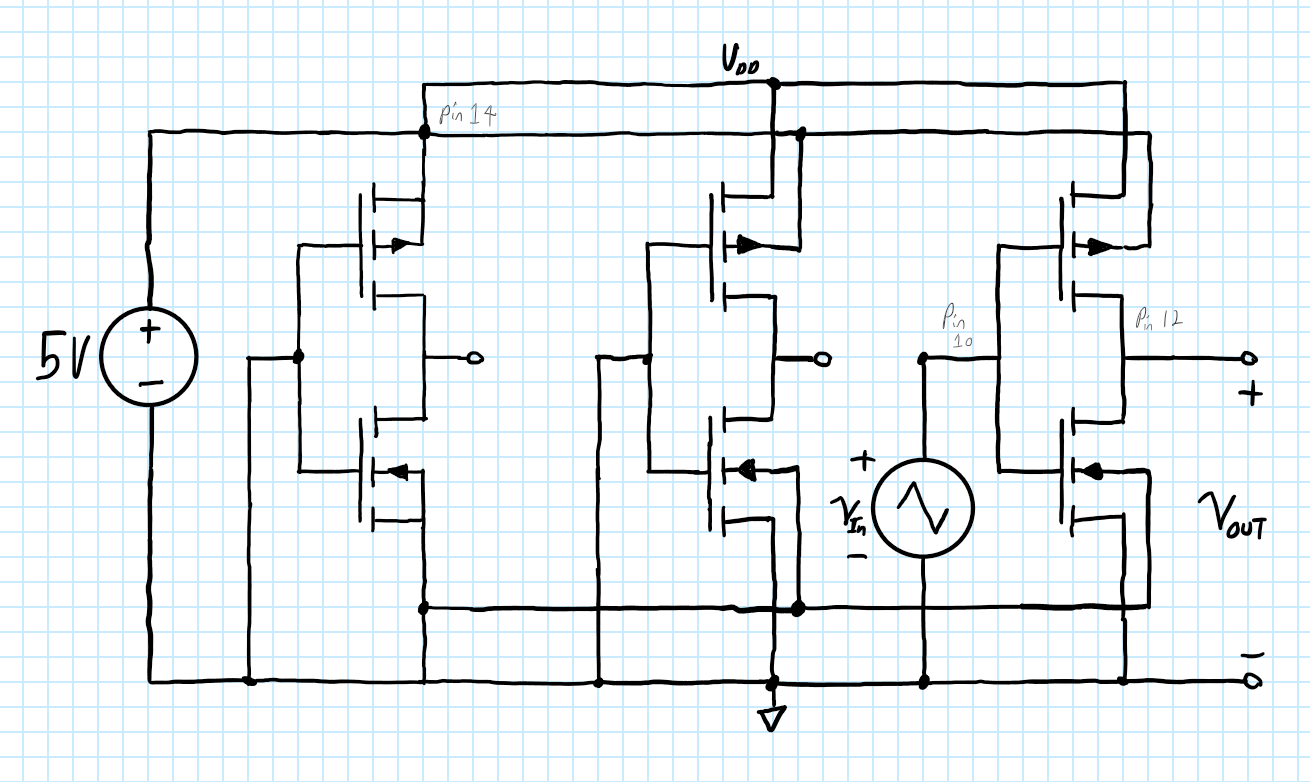
\includegraphics[scale=0.35]{singleInverter.png}
\end{center}

using the CD4007UB integrated circuit, and measuring $v_{in}$ at the function generator and $v_{out}$ at pin 12 and ground.\\
$V_{DD}$ was set to 5V DC, and $v_{in}$ was a 500 Hz 0V to 5V triangle wave.\\

\textbf{Step 6}\\
The oscilloscope display was captured showing $v_{in}$ and $v_{out}$ as signals. The oscilloscope display was then changed 
to be in XY mode, such that $v_{in}$ represented the horizontal axis, and $v_{out}$ represented the vertical axis.\\


\subsection*{Results / Calculations}

\textbf{Step 6}\\

The following screenshot shows $v_{in}$ and $v_{out}$ displayed as 2 channels in normal time mode.\\

\begin{center}
    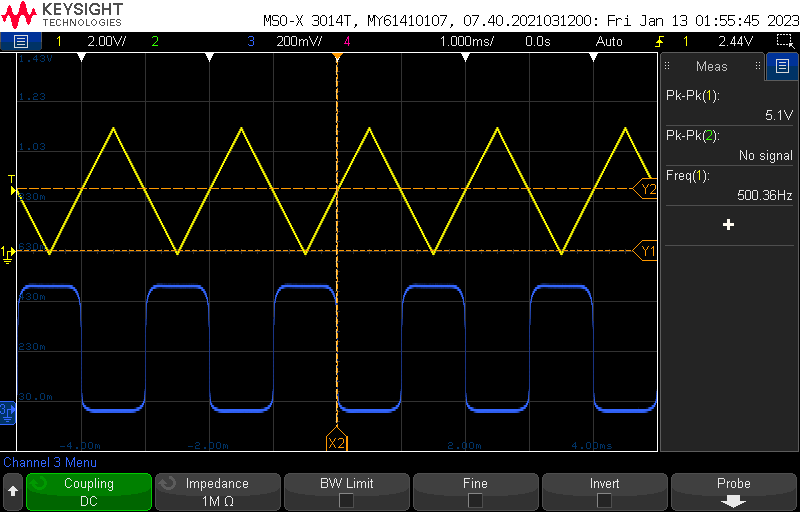
\includegraphics[scale=0.5]{scope2.png}
\end{center}

\textbf{Step 7}\\

\vspace{4pt}
The below graph represents the transfer characteristic $v_{out}$ vs. $v_{in}$, with points labeled to represent
what mode the transistor is in, and which voltages correlate with those descriptions.\\

\begin{center}
    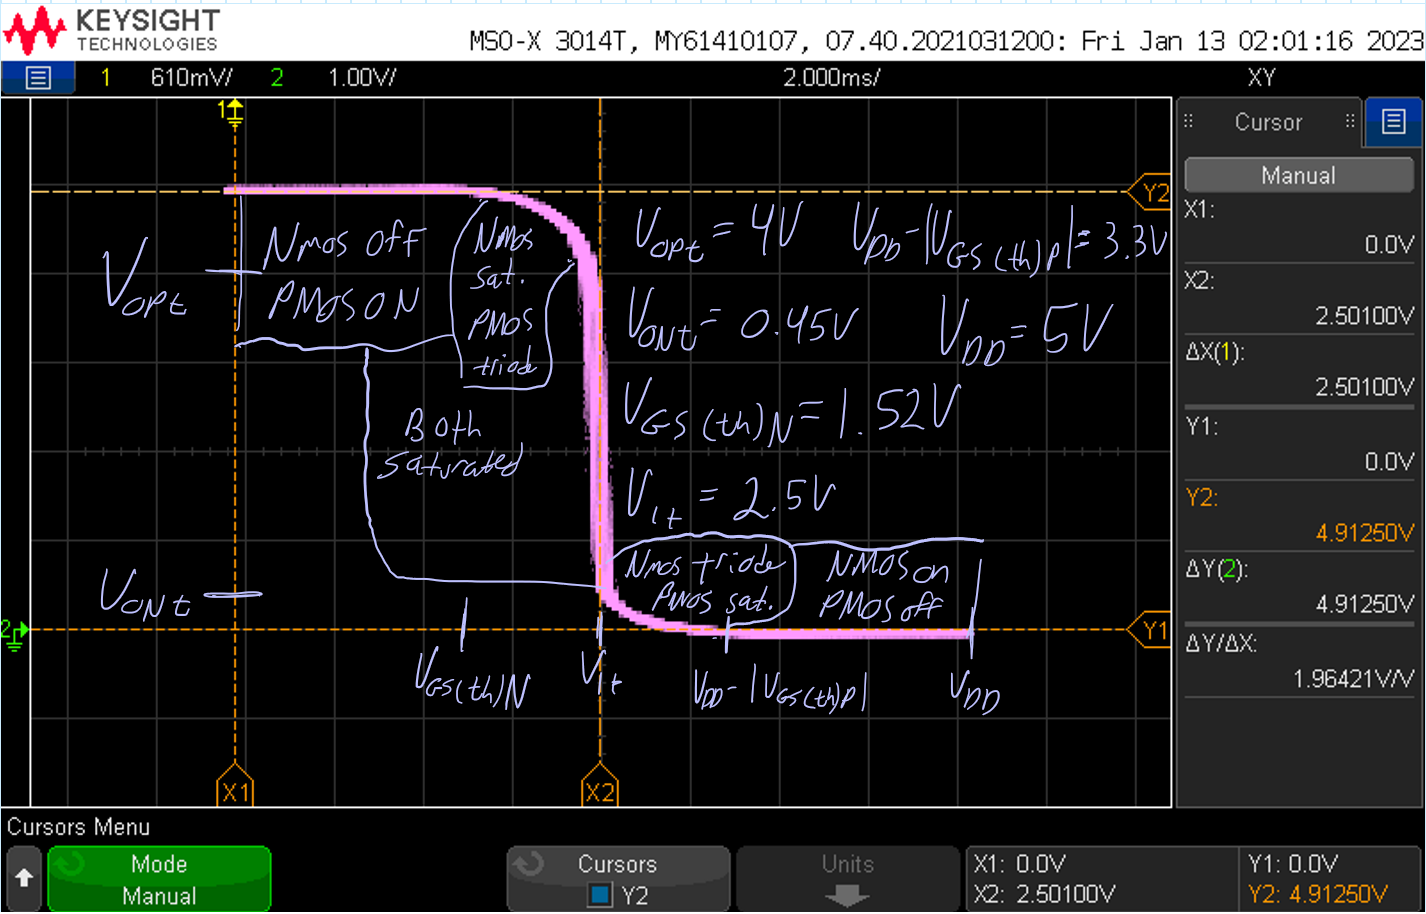
\includegraphics[scale=0.4]{scope3.png}
\end{center}

\vspace{7pt}

\textbf{Step 8}\\

The below graph depicts the transfer characteristic ${v_{out}}$ vs. $v_{in}$, with noise margins and their voltages
labeled.\\

\begin{center}
    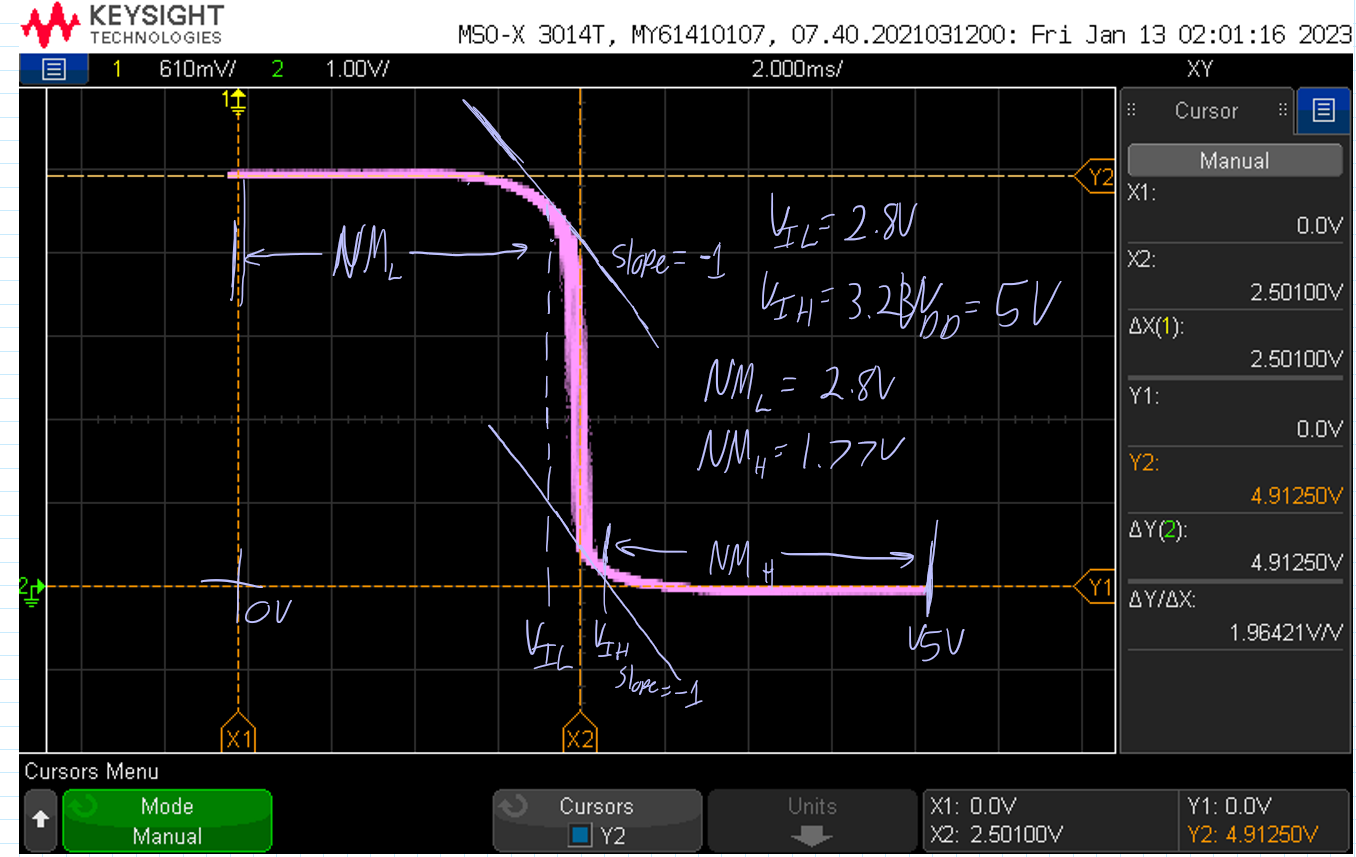
\includegraphics[scale=0.4]{scope4.png}
\end{center}

The noise margins defined on the datasheet for the CD4007UB transistor chip show that the worst-case margins 
are $V_{IL}$ = 4.5V, and $V_{IH}$ = 0.5V.\\

\subsection*{Conclusions}

\indent\indent In this section, a simple inverter circuit was demonstrated with a CD4007UB integrated circuit containing
three complimentary pairs of NMOS and PMOS transistors. The transfer characteristic was found, and various intrinsic properties 
of this characteristic were determined and shown to be within limits and reasonable values. \\

\section*{Task 3}

\subsection*{Objective}
\indent\indent The objective of this task is to create a ring oscillator by daisy-chaining 3 inverters in a loop, 
and to find its oscillation frequency and propagation delay of the inverter circuit.\\

\subsection*{Procedure}

\subsection*{Results / Calculations}

\subsection*{Conclusions}
\newpage

\printbibliography[title={\Large References}] %Prints out the bibliography sources that you have used in the document.

\end{document}